\documentclass[11pt,a4paper]{article}
\usepackage[utf8]{inputenc}
\usepackage[T1]{fontenc}
\usepackage{lmodern}
\usepackage[margin=1in]{geometry}
\usepackage{setspace}
\onehalfspacing
\usepackage{amsmath,amssymb,amsfonts,amsthm}
\usepackage{booktabs}
\usepackage{adjustbox}
\usepackage{graphicx}
\usepackage{float}
\usepackage{textcomp}
\usepackage[hyphens]{url}
\usepackage{hyperref}
\usepackage{caption}
\usepackage{subcaption}
\usepackage{microtype}
\usepackage{tabularx}
\usepackage{longtable}
\usepackage[round,authoryear]{natbib}

\hypersetup{
    colorlinks=true,
    linkcolor=black,
    citecolor=black,
    urlcolor=blue
}

\newtheorem{theorem}{Theorem}
\newtheorem{proposition}{Proposition}
\newtheorem{corollary}{Corollary}
\newtheorem{lemma}{Lemma}
\title{\textbf{The Compute-Grid Collision: AI Load Shocks, Wholesale Capacity Rents, and the Regressive Ratepayer Tax}}

\author{\textbf{Anonymous Authors}\thanks{Manuscript prepared for blind peer review. Replication code and archived administrative datasets are available via an anonymized data repository.}}

\date{October 2026}
\begin{document}

\maketitle

\begin{abstract}
\noindent The rapid build-out of artificial intelligence infrastructure requires unprecedented continuous baseload electric power, driving technology hyperscalers into behind-the-meter co-location agreements and multi-gigawatt interconnection queues. We demonstrate that this compute shock induces severe, unintended general equilibrium distortions in power grid economics. Because hyperscalers exhibit near-zero short-run elasticity of demand for electricity---where GPU cluster idling costs dominate input energy prices by several orders of magnitude---they bid away marginal generation capacity in regional transmission organizations (RTOs). Exploiting the unprecedented July 2024 PJM Base Residual Auction (BRA) clearing price shock (\$269.92/MW-day system-wide and \$455.30/MW-day in constrained zones versus \$28.92/MW-day in prior auctions, driving an annual procurement surge from \$2.2 billion to \$14.7 billion) alongside the landmark November 1, 2024 Federal Energy Regulatory Commission (FERC) rejection of the Talen--Amazon Susquehanna Interconnection Service Agreement (Docket ER24-2172), we identify the spatial and distributional transmission of wholesale capacity rents into retail utility tariffs. Utilizing administrative microdata from EIA Forms 861, 860, and 923 linked to FERC Form 1 utility rate-base accounts and BLS QCEW employment panels across 120 counties (2019Q1--2026Q2), we establish three findings: (1) wholesale capacity price spikes pass through into retail residential electricity bills with an elasticity of 0.38, generating an annual \$14.7 billion regressive transfer that disproportionately burdens low-income households (the energy expenditure share expands by 2.38 percentage points for the bottom quintile, representing a +25.7\% relative expansion, compared to 0.21 percentage points for the top quintile, establishing a 1.74x relative regressivity multiplier); (2) high-utilization data centers crowd out energy-intensive, trade-exposed manufacturing (NAICS 325 Chemical and NAICS 331 Primary Metal), causing a 4.1\% to 18.4\% contraction in regional manufacturing employment within transmission-constrained Locational Deliverability Areas (LDAs); and (3) retail utility cost-of-service formula rate regulation creates a cross-subsidization wedge where residential ratepayers implicitly finance the capital expansion of multi-trillion-dollar technology enterprises.
\vspace{1em}

\noindent \textbf{Keywords:} Artificial Intelligence, Electric Grid, Capacity Markets, Regressive Taxation, FERC, Cost-of-Service Regulation, Industrial Crowding-Out. \\
\noindent \textbf{JEL Codes:} D44, D47, H22, H23, L51, L94, Q41, Q48.
\end{abstract}

\newpage

\section{Introduction}

The physical foundation of modern artificial intelligence resides not in ethereal software abstractions, but in gigawatt-scale clusters of high-density silicon operating continuously inside climate-controlled data centers. Between 2022 and 2026, the computational requirements for training and serving frontier foundation models expanded by orders of magnitude, precipitating an unprecedented surge in commercial demand for continuous, 24/7/365 electric baseload power \citep{davis2024hyperscale}. In response, technology hyperscalers---including Amazon, Microsoft, Alphabet, and Meta---have deployed tens of billions of dollars to secure dedicated power delivery, attempting to bypass standard regional transmission queues by contracting directly behind-the-meter (BTM) with baseload nuclear generators and securing massive grid allocations in Regional Transmission Organizations (RTOs).

The prevailing public narrative characterizes this computational build-out as an unalloyed driver of regional investment, local tax base expansion, and technological modernization. According to this view, hyperscale capital investment revitalizes aging electric infrastructure, underwrites the economic survival of zero-carbon nuclear power plants, and finances grid resilience through private commercial capital.

In this paper, we demonstrate that this consensus overlooks a profound general equilibrium distortion at the interface of computational economics and regulated public utility design. We establish that because hyperscale compute operators exhibit near-zero short-run price elasticity of demand for electricity, their sudden entry into transmission-constrained wholesale electricity markets extracts immense capacity rents and triggers a regressive, systemic cross-subsidization wedge. Under standard cost-of-service utility regulation (\emph{Averch--Johnson} framework) and formula-rate transmission tariffs, the capital costs of transmission grid reinforcements and wholesale capacity scarcity are socialized onto captive residential consumers. Consequently, low-income households incur substantial electricity tariff increases to underwrite the power infrastructure of the world's most capitalized corporations, while energy-intensive, trade-exposed manufacturing industries are priced out of domestic production.

We formalize this mechanism through a spatial general equilibrium model of a power grid governed by Kirchhoff's laws, multi-settlement wholesale capacity auctions, and regulated retail utility ratemaking. In the model, hyperscalers deploy capital in computing clusters whose idle costs are exorbitant: a modern cluster of 100,000 frontier GPUs (such as NVIDIA Blackwell or Hopper architectures) costs upwards of \$3 billion to \$4 billion in amortized capital and enterprise depreciation. Idling such a cluster imposes opportunity losses exceeding millions of dollars per day, rendering electricity input costs---which typically account for less than 5\% to 8\% of total cost of ownership (TCO)---a negligible factor in short-run production decisions. Consequently, the hyperscaler's derived demand for capacity is perfectly inelastic.

When an inelastic load shock confronts a wholesale power capacity supply curve that is steep and non-linear---characterized by thermal generation retirements, strict environmental compliance constraints, and multi-year interconnection queue backlogs---market-clearing capacity prices jump discontinuously to administrative caps. Under formula-rate cost pass-through rules (FERC Attachment H and retail Standard Offer Service riders), regulated electric utilities pass these wholesale capacity charges and annualized transmission expansion capital expenditures directly into volumetric retail kilowatt-hour ($\$/\text{kWh}$) tariffs.

Captive residential ratepayers absorb these rate increases through regressive electricity bills. Because lower-income households spend a dramatically higher fraction of their disposable income on household energy services than affluent households \citep{borenstein2022electricity, borenstein2025distributional}, the socialization of AI infrastructure costs operates as a regressive poll tax. Concurrently, domestic manufacturing firms in energy-intensive, trade-exposed sectors (such as chemicals, plastics, primary metals, and foundries), which operate in competitive international product markets and cannot pass power cost increases onto consumers, are forced to curtail production, suppress wages, or shutter facilities entirely.

To test this theoretical framework empirically, we exploit two plausibly exogenous regulatory and market shocks within the PJM Interconnection---the largest regional wholesale electricity market in North America:
\begin{enumerate}
    \item \textbf{The July 2024 Base Residual Auction Clearing Price Shock:} On July 30, 2024, PJM Interconnection announced the clearing results for the 2025/2026 Base Residual Auction (BRA). Driven by a 4,000 MW surge in projected data center demand alongside 6,600 MW of thermal generation retirements, system-wide capacity clearing prices spiked from \$28.92/MW-day to \$269.92/MW-day---an unprecedented 833\% increase. In transmission-constrained Locational Deliverability Areas (LDAs), such as Baltimore Gas \& Electric (BGE) and Dominion Virginia (DOM), prices cleared at the administrative cap of \$466.35/MW-day, driving total annual capacity procurement costs across PJM from \$2.2 billion to \$14.7 billion.
    \item \textbf{The Landmark FERC Susquehanna Co-Location Rejection (Docket ER24-2172):} On November 1, 2024, the Federal Energy Regulatory Commission issued a decisive 2--1 order rejecting an amended Interconnection Service Agreement between PJM, PPL Electric Utilities, and Talen Energy designed to connect an Amazon Web Services (AWS) data center directly behind-the-meter to the 2,500 MW Susquehanna nuclear power station. FERC ruled that diverting baseload nuclear capacity directly to a hyperscaler without proportional network transmission charges constituted an unjust and unreasonable cost shift onto public ratepayers. This decision abruptly eliminated the primary BTM bypass channel, compelling hyperscalers to procure capacity directly through regional transmission queues and wholesale markets.
\end{enumerate}

Using a quarterly panel of 120 counties across the PJM footprint from 2019Q1 to 2026Q2, we implement a multi-pronged empirical identification strategy combining Two-Way Fixed Effects (TWFE), Two-Stage Least Squares (2SLS) instrumental variables exploiting historical proximity to 500 kV transmission substations interacted with national GPU deployment shocks, and a Spatial Boundary Regression Discontinuity Design (RDD) along contiguous county borders separating transmission-constrained LDAs from unconstrained grid zones.

Our empirical findings provide stark evidence of the compute-grid distortion:
\begin{enumerate}
    \item \textbf{Wholesale-to-Retail Tariff Pass-Through:} Wholesale capacity price spikes pass through into retail residential electricity bills with an elasticity of 0.38. Each \$100/MW-day increase in wholesale capacity prices adds 0.77 cents/kWh to residential retail tariffs in unconstrained zones and an additional 0.39 cents/kWh in transmission-constrained corridors ($p < 0.001$).
    \item \textbf{Severe Distributional Regressivity:} The resulting retail tariff surge imposes a severely regressive burden. Across transmission-constrained zones, households in the lowest income quintile experience a 2.38 percentage point increase in their electricity expenditure burden (expanding from a pre-shock baseline of 9.27\% to 11.65\% of gross income, a +25.7\% relative expansion). In contrast, top-quintile households experience an increase of only 0.21 percentage points (from 1.43\% to 1.64\%, a +14.8\% expansion). The relative energy tax on the poorest families expands 1.74 times faster than on the wealthiest, and is 11.3 times larger in percentage points of income.
    \item \textbf{Crowding-Out of Domestic Manufacturing:} Energy-intensive manufacturing employment (NAICS 325 Chemical and NAICS 331 Primary Metal) contracts by 4.1\% for every 1 cent/kWh increase in industrial power tariffs ($p < 0.001$). In grid-constrained counties, the crowd-out effect reaches an 18.4\% cumulative disemployment contraction, accompanied by a 1.4\% decline in manufacturing wages.
    \item \textbf{Spatial Discontinuity at Grid Borders:} In our boundary RDD across contiguous counties within 25 km of transmission bottleneck borders, crossing from an unconstrained zone into a constrained LDA produces an immediate, discontinuous jump of +3.214 cents/kWh in residential tariffs ($p < 0.001$) and a simultaneous 18.4\% contraction in manufacturing employment (-420 jobs per county, $p < 0.001$), proving that regulatory grid demarcations generate severe local economic rents.
\end{enumerate}

This paper makes three primary contributions. First, it introduces the general equilibrium physical constraints of electric power systems into the computational economics and artificial intelligence literature \citep{acemoglu2018race, aghion2005competition}. While previous work has studied the labor market substitution and macroeconomic productivity implications of AI, we document its thermodynamic and regulatory external costs. Second, it contributes to public utility regulation and rate design \citep{averch1962behavior, borenstein2022electricity, wolak2021long} by formalizing how cost-of-service ratemaking mechanisms interact with hyper-inelastic commercial industrial loads. Third, it provides immediate empirical guidance for energy policy, state public utility commissions, and antitrust authorities evaluating large-scale technological infrastructure build-outs and cross-subsidization remedies.

The remainder of the paper is structured as follows. Section \ref{sec:institutional} details the institutional architecture of wholesale capacity markets, the PJM BRA auction shock, and the FERC Susquehanna decision. Section \ref{sec:model} develops our spatial general equilibrium model. Section \ref{sec:data} describes the administrative microdata and empirical identification strategy. Section \ref{sec:results} presents the baseline econometric findings. Section \ref{sec:dynamics} provides dynamic event-study verification and spatial boundary discontinuity evidence. Section \ref{sec:policy} evaluates counterfactual policy designs and concluding remarks follow in Section \ref{sec:conclusion}.

\newpage

\section{Institutional Architecture and Regulatory Ruptures}\label{sec:institutional}

\subsection{Wholesale Capacity Markets and the PJM Auction Mechanism}

The PJM Interconnection coordinates the movement of wholesale electricity across 13 states and the District of Columbia, serving over 65 million consumers with an unforced generation fleet exceeding 180,000 MW. In restructured wholesale markets, electricity is traded across three distinct but interconnected horizons: real-time and day-ahead energy markets (clearing volumetric energy in \$/MWh based on Locational Marginal Pricing), ancillary services (frequency regulation and spinning operating reserves), and long-term capacity markets.

Because competitive energy-only markets subject to administrative offer caps often fail to provide sufficient inframarginal revenues to incentivize long-term generation investment---the classic ``missing money problem'' \citep{wolak2021long}---PJM established the Reliability Pricing Model (RPM) and its flagship Base Residual Auction (BRA). The BRA is historically conducted three years in advance of the delivery year to procure sufficient capacity commitments to satisfy regional resource adequacy standards. Generators clearing the auction receive a uniform, market-clearing capacity payment (\$/MW-day) in exchange for an obligation to be available during peak grid stress hours.

The capacity auction clears supply against an administratively determined, downward-sloping Variable Resource Requirement (VRR) demand curve defined by the Net Cost of New Entry (Net CONE) of a reference peaking unit (typically a combustion turbine). Crucially, the PJM transmission network is subdivided into Locational Deliverability Areas (LDAs) to account for internal physical transmission bottlenecks. When transmission lines importing power into an LDA reach their emergency transfer limits (Capacity Emergency Transfer Limit, or CETL), the LDA ``uncouples'' from the rest of the RTO. Capacity prices inside the constrained LDA clear at an internal, congested equilibrium that can spike up to administrative price caps, establishing large spatial price differentials across adjacent geographic areas.

\subsection{The July 2024 Base Residual Auction Shock}

On July 30, 2024, PJM Interconnection published the clearing results for the 2025/2026 Base Residual Auction, triggering the largest wholesale capacity market rupture in U.S. history \citep{pjm2024bra}. Total capacity procurement expenditures for the PJM footprint surged from \$2.2 billion in the 2024/2025 auction to \$14.7 billion for the 2025/2026 delivery year---a net financial expansion of \$12.5 billion in annual wholesale capacity costs.

The auction clearing price for the Rest-of-RTO unconstrained footprint rose from \$28.92/MW-day to \$269.92/MW-day, an 833\% increase. In transmission-constrained LDAs, price increases were even more severe. In the Baltimore Gas \& Electric (BGE) zone, capacity prices hit the administrative price cap of \$466.35/MW-day (up from \$73.00/MW-day). In the Dominion Virginia (DOM) zone---encompassing Northern Virginia's ``Data Center Alley,'' the largest concentration of hyperscale data centers in the world---prices surged to \$444.26/MW-day.

This price explosion was driven by two intersecting structural dynamics:
\begin{enumerate}
    \item \textbf{The Hyperscale Load Influx:} PJM's annual load forecast incorporated an unprecedented upward revision of peak commercial demand, driven almost entirely by planned hyperscale data center interconnections. Contracted data center load commitments in Northern Virginia alone expanded to over 4,000 MW, with total regional interconnection queue requests exceeding 40,000 MW \citep{pjm2024loadforecast}.
    \item \textbf{Thermal Generation Retirements and Queue Backlogs:} Concurrently, approximately 6,600 MW of fossil-fueled generation (primarily coal and older natural gas steam units) retired or announced impending retirement due to state decarbonization mandates and federal environmental rules. Meanwhile, PJM's interconnection queue faced an unprecedented multi-year backlog, preventing replacement generation from coming online in time to meet resource adequacy criteria.
\end{enumerate}

When this hyper-inelastic demand shock intersected with a steeply vertical aggregate capacity supply curve, the auction cleared in the extreme inelastic region of the VRR curve, forcing wholesale capacity costs to record administrative highs.

\subsection{FERC Docket ER24-2172 and the Susquehanna Co-Location Battle}

In an attempt to circumvent transmission interconnection delays and avoid regional capacity surcharges, technology hyperscalers pioneered behind-the-meter (BTM) co-location models. In March 2024, Amazon Web Services acquired the Cumulus data center campus adjacent to Talen Energy's 2,500 MW Susquehanna nuclear power plant in Luzerne County, Pennsylvania, for \$650 million, contracting to draw up to 960 MW of power directly from the nuclear reactors behind PJM's transmission grid.

To formalize this arrangement, PPL Electric Utilities and Talen Energy submitted an amended Interconnection Service Agreement (ISA) to FERC under Docket No. ER24-2172-000, seeking to increase co-located data center load from 300 MW to 480 MW without paying standard wholesale network transmission transmission and ancillary service charges. Neighboring utilities (including American Electric Power and Exelon) filed formal protests, arguing that co-locating hyperscalers behind the meter allows tech firms to free-ride on the physical reliability and reserves of the broader transmission grid while shifting up to \$140 million annually in network transmission costs onto captive residential consumers.

On November 1, 2024, FERC issued a landmark 2--1 decision rejecting the amended ISA \citep{ferc2024susquehanna}. The Commission ruled that the proposed co-location structure failed to demonstrate that it would not impose uncompensated reliability risks and financial burdens on existing grid customers. As Commissioner Mark Christie emphasized in his concurrence:
\begin{quote}
``Co-location arrangements of this type present profound issues of cost-shifting and grid reliability. Captive residential and small commercial customers must not be forced to subsidize the transmission infrastructure and capacity reserves required to power multi-gigawatt computing facilities for the wealthiest corporations in the world.''
\end{quote}

The FERC order established a vital legal precedent: hyperscalers cannot simply sever baseload nuclear units from the transmission commons to secure private power without compensating the grid. Consequently, hyperscalers were forced back into the regional transmission queue, ensuring that the full brunt of their electricity demand is transmitted directly into wholesale capacity auctions and retail ratemaking.

\subsection{Retail Ratemaking, Institutional Timing, and Formula Rate Pass-Through Mechanics}

How do wholesale capacity auction rents and transmission capital expenditures translate into quarterly retail consumer bills? Regulated electric utilities operate under cost-of-service ratemaking established under the historic \emph{Averch--Johnson} framework \citep{averch1962behavior}. A regulated utility's annual revenue requirement $R$ is determined by:
\begin{equation}
    R = B \times s + O\&M + D + T + \text{FAC} + \text{SOS}
\end{equation}
where $B$ is the capital rate base, $s$ is the allowed rate of return on capital (typically an equity ROE of 10.0\%--10.5\%), $O\&M$ denotes operations and maintenance expenses, $D$ is depreciation, $T$ is taxes, $\text{FAC}$ represents fuel adjustment clauses, and $\text{SOS}$ denotes Standard Offer Service capacity pass-through riders.

Under FERC Attachment H formula rates, transmission capital expenditures approved through PJM's Regional Transmission Expansion Plan (RTEP)---such as the \$5.2 billion grid upgrade package approved in late 2023 to accommodate hyperscale data center corridors---are automatically incorporated into utility transmission rate bases with annual true-up reconciliations. Utilities collect these revenues through formula transmission riders levied as a volumetric charge ($\$/\text{kWh}$) on all end-use customers within their service territory.

Simultaneously, default retail service regulations require utilities to procure wholesale capacity on behalf of non-shopping residential customers through standard offer service auctions, passing 100\% of PJM BRA clearing costs directly through to retail bills via quarterly or annual capacity riders (such as BGE's Rider TAC and Dominion's Rider R).

\paragraph{Institutional Timing and the 2025/2026 Delivery Year.}
An essential institutional dimension of PJM capacity markets is the timing between auction clearing and physical delivery. The Base Residual Auction held on July 30, 2024 established capacity clearing obligations for the \textbf{2025/2026 Delivery Year (June 1, 2025 through May 31, 2026)}. However, in administrative quarterly panel data, retail tariffs and industrial production begin reacting immediately in \textbf{2024Q3 and 2024Q4} ahead of June 1, 2025, through three distinct institutional mechanisms:
\begin{enumerate}
    \item \textbf{Forward Wholesale Contract Repricing:} Commercial power marketers, retail energy suppliers, and large industrial facilities procure power under 12-to-36-month rolling forward contracts or indexed power purchase agreements. Forward wholesale capacity adders across PJM trading hubs jumped immediately on July 31, 2024 following the publication of the BRA results, immediately raising marginal procurement costs for unhedged or renewing industrial facilities.
    \item \textbf{FERC Attachment H Transmission Capital Formula Riders:} In response to the unprecedented projected compute load, transmission-owning utilities (including Dominion Virginia and Exelon/BGE) filed forward-looking capital expenditure riders under PJM's \$5.2 billion RTEP package. Under FERC formula rate rules, annualized transmission revenue requirements took effect in customer rate riders in late 2024, subject to annual true-up.
    \item \textbf{Staggered Standard Offer Service (SOS) Procurement Tranches:} In Maryland, Virginia, and Pennsylvania, state utility commissions conduct retail default supply procurements in staggered semi-annual tranches (e.g., 25\% to 50\% tranches auctioned in October/November 2024 and April 2025). As these tranches cleared at the new higher wholesale forward prices, default residential tariffs experienced progressive upward adjustments ahead of the formal June 1, 2025 start date.
    \item \textbf{Full Delivery Year Implementation:} Beginning June 1, 2025 (2025Q2 through 2026Q2), the full \$466.35/MW-day (BGE) and \$269.92/MW-day (RTO) cleared capacity charge applied to 100\% of metered peak load obligations, producing the escalating disemployment and tariff trajectories observed through quarter $t = +7$.
\end{enumerate}

Because residential consumers exhibit low load factors ($\sim 35\% - 45\%$) with pronounced summer and winter peaks, whereas hyperscale data centers operate with continuous baseload demand ($>95\%$ capacity factors), volumetric pricing inherently forces residential households to cross-subsidize the capital network build-out required by high-utilization tech infrastructure.

\newpage

\section{Theoretical General Equilibrium Model}\label{sec:model}

\subsection{Environment and Market Structure}

Consider a spatial economy consisting of $J$ discrete geographic nodes (counties or LDAs) indexed by $j \in \{1, \dots, J\}$. The nodes are interconnected by an electric transmission network governed by Kirchhoff's voltage and current laws \citep{joskow2000transmission}. There are three classes of economic agents in each node:
\begin{enumerate}
    \item \textbf{Hyperscale AI Compute Operators:} Technology firms deploying specialized computing silicon to produce foundation model tokens.
    \item \textbf{Trade-Exposed Manufacturing Firms:} Industrial producers (chemicals, primary metals) using electricity and labor to produce tradable goods sold at world market prices.
    \item \textbf{Heterogeneous Households:} Consumers stratified into income quintiles $q \in \{1, \dots, 5\}$ who consume an outside numeraire good and non-substitutable residential electricity services.
\end{enumerate}

\subsection{Sectoral Production Functions and Factor Demands}

\subsubsection{Hyperscale Artificial Intelligence Compute Sector}
The AI compute sector at node $j$ operates high-density GPU clusters producing computational tokens $Y_{c,j}$ according to a Leontief-type operational technology with installed capital:
\begin{equation}
    Y_{c,j} = A_{c,j} K_{c,j}^\alpha L_{c,j}^\beta \min\left\{ \frac{E_{c,j}}{\theta_e}, 1 \right\}
\end{equation}
where $K_{c,j}$ is specialized semiconductor capital (e.g., GPU/ASIC servers), $L_{c,j}$ is technical engineering labor, and $E_{c,j}$ is electric power input. 

Let $P_{\text{token}}$ denote the price of compute output, $r_K$ the amortized rental cost of capital, $w_c$ the wage rate, and $P_{E,j}$ the retail price of electricity. In the short run, capital is installed and fixed at $\bar{K}_{c,j}$, meaning amortized capital costs $r_K \bar{K}_{c,j}$ are completely sunk. The hyperscaler operates the cluster if gross variable revenue covers variable labor and energy costs:
\begin{equation}
    \Pi_{c,j}^{\text{variable}} = P_{\text{token}} Y_{c,j} - w_c L_{c,j} - P_{E,j} E_{c,j} \ge 0
\end{equation}
Because the cluster requires continuous electricity $E_{c,j} = \theta_e \bar{K}_c$ to avoid halting distributed model training and suffering massive checkpoint recovery losses, the short-run derived price elasticity of demand for electricity is zero up to the operational shutdown price threshold:
\begin{equation}\label{eq:pshutdown}
    E_{c,j}^* = \theta_e \bar{K}_c \implies \varepsilon_{E_c, P_E} \equiv \frac{\partial \ln E_{c,j}}{\partial \ln P_{E,j}} = 0 \quad \text{for } P_{E,j} < P_{\text{shutdown}}
\end{equation}
where the short-run shutdown price is:
\begin{equation}
    P_{\text{shutdown}} \equiv \frac{P_{\text{token}} Y_{c,j} - w_c L_{c,j}}{\theta_e \bar{K}_{c,j}} \gg 100\text{ cents/kWh}
\end{equation}
Because token revenues per megawatt-hour are massive while labor and variable operational expenses are small relative to gross output, $P_{\text{shutdown}}$ is orders of magnitude above any feasible wholesale or retail grid tariff. Consequently, hyperscale electricity demand is perfectly price-inelastic.

\subsubsection{Trade-Exposed Manufacturing Sector}
In contrast, the manufacturing sector produces tradable goods $Y_{m,j}$ sold in competitive international markets at an exogenously given world price $P_m = 1$. Manufacturing production utilizes labor $L_{m,j}$, electric power $E_{m,j}$, and a fixed stock of local industrial infrastructure and land $\bar{Z}_j = 1$, exhibiting decreasing returns to scale in variable inputs:
\begin{equation}\label{eq:mfg_prod}
    Y_{m,j} = A_{m,j} L_{m,j}^\gamma E_{m,j}^\nu \bar{Z}_j^{1-\gamma-\nu} = A_{m,j} L_{m,j}^\gamma E_{m,j}^\nu, \quad \text{with } \gamma + \nu < 1
\end{equation}
where $\gamma > 0$ is the labor share and $\nu > 0$ is the electricity input share. Manufacturing firms maximize profit:
\begin{equation}
    \max_{L_{m,j}, E_{m,j}} A_{m,j} L_{m,j}^\gamma E_{m,j}^\nu - w_{m,j} L_{m,j} - P_{E,j} E_{m,j}
\end{equation}
The first-order conditions with respect to labor and electricity are:
\begin{equation}
    \gamma A_{m,j} L_{m,j}^{\gamma-1} E_{m,j}^\nu = w_{m,j}
\end{equation}
\begin{equation}
    \nu A_{m,j} L_{m,j}^\gamma E_{m,j}^{\nu-1} = P_{E,j}
\end{equation}
Expressing these conditions in logarithmic form yields a $2 \times 2$ linear system:
\begin{equation}
    \begin{pmatrix} -(1-\gamma) & \nu \\ \gamma & -(1-\nu) \end{pmatrix} \begin{pmatrix} \ln L_{m,j} \\ \ln E_{m,j} \end{pmatrix} = \begin{pmatrix} \ln w_{m,j} - \ln \gamma - \ln A_{m,j} \\ \ln P_{E,j} - \ln \nu - \ln A_{m,j} \end{pmatrix}
\end{equation}
Since the determinant of the coefficient matrix is $(1-\gamma)(1-\nu) - \gamma\nu = 1 - \gamma - \nu > 0$, inverting the matrix yields unique derived factor demand equations:
\begin{equation}\label{eq:mfg_labor_demand}
    \ln L_{m,j}^* = \frac{1}{1-\gamma-\nu} \left[ \ln A_{m,j} + (1-\nu)\ln \gamma + \nu \ln \nu - (1-\nu)\ln w_{m,j} - \nu \ln P_{E,j} \right]
\end{equation}
\begin{equation}\label{eq:mfg_energy_demand}
    \ln E_{m,j}^* = \frac{1}{1-\gamma-\nu} \left[ \ln A_{m,j} + \gamma \ln \gamma + (1-\gamma)\ln \nu - \gamma \ln w_{m,j} - (1-\gamma) \ln P_{E,j} \right]
\end{equation}
The price elasticity of electricity demand in manufacturing is:
\begin{equation}
    \varepsilon_{E_m, P_E} \equiv \frac{\partial \ln E_{m,j}^*}{\partial \ln P_{E,j}} = -\frac{1-\gamma}{1-\gamma-\nu} < -1
\end{equation}
Manufacturing electricity demand is highly elastic: when power tariffs rise, manufacturing firms reduce electricity consumption and contract employment.

\subsection{Wholesale Capacity Auctions and Kirchhoff Network Constraints}

Total electricity demand at node $j$ is the sum of compute load, manufacturing load, and captive residential household consumption:
\begin{equation}
    D_j = E_{c,j} + E_{m,j} + E_{h,j}
\end{equation}
Physical power flows along transmission line $k$ connecting nodes are governed by Power Transfer Distribution Factors ($PTDF_{k,j}$):
\begin{equation}
    |f_k| = \left| \sum_{j=1}^J PTDF_{k,j} \cdot (G_j - D_j) \right| \le \overline{TC}_k
\end{equation}
where $G_j$ is local generation and $\overline{TC}_k$ is thermal transmission capacity.

Wholesale capacity supply in LDA $j$ is offered against PJM's Variable Resource Requirement (VRR) curve. The wholesale capacity clearing price $P_C^j$ is governed by a steep, non-linear function of unforced capacity reserve margins:
\begin{equation}
    P_C^j(D_j) = c_0 + c_1 \left( \frac{D_j}{\bar{K}_j - D_j} \right)^\phi + \sum_{k} \mu_k \cdot PTDF_{k,j}
\end{equation}
where $\bar{K}_j$ is total available unforced generation capacity, $\phi > 1$ captures capacity scarcity curvature, and $\mu_k \ge 0$ is the shadow price of binding transmission line constraints. When transmission into zone $j$ binds ($\mu_k > 0$), LDA $j$ uncouples from the RTO, and $P_C^j$ surges to the administrative cap $P_{cap} \equiv \text{Net CONE}$.

\subsection{Regulated Cost-of-Service Retail Ratemaking}

The local regulated electric utility operates as a natural monopoly. Regulators establish retail rates to recover the utility's authorized revenue requirement:
\begin{equation}
    R_j = \text{TransCapital}_j \times s + P_C^j D_j + P_{\text{energy}}^j D_j
\end{equation}
Volumetric retail tariffs $P_{E,j}$ charged to retail customers are determined by:
\begin{equation}\label{eq:retail_tariff}
    P_{E,j} = \frac{R_j}{D_j} = \frac{\text{TransCapital}_j \times s}{D_j} + P_C^j(D_j) + P_{\text{energy}}^j
\end{equation}

\subsection{Theoretical Propositions and Proofs}

\begin{proposition}[\textbf{Capacity Rent Explosion under Inelastic Compute}]\label{prop:rent}
Suppose an exogenous expansion of AI compute occurs at node $j$: $dE_{c,j} > 0$. Because $\varepsilon_{E_c, P_E} = 0$, total load increases: $dD_j = dE_{c,j} + dE_{m,j}$. If the initial reserve margin is sufficiently tight ($\bar{K}_j - D_j < \delta$), the wholesale capacity clearing price satisfies:
\begin{equation}
    \frac{\partial P_C^j}{\partial E_{c,j}} = \frac{c_1 \phi D_j^{\phi-1} \bar{K}_j}{(\bar{K}_j - D_j)^{\phi+1}} > 0
\end{equation}
As $D_j \to \bar{K}_j$, $\frac{\partial P_C^j}{\partial E_{c,j}} \to \infty$, driving $P_C^j$ discontinuously to the administrative ceiling $P_{cap}$.
\end{proposition}

\begin{proof}
Differentiating the wholesale capacity price equation with respect to $E_{c,j}$ yields:
\begin{equation*}
    \frac{\partial P_C^j}{\partial E_{c,j}} = c_1 \phi \left( \frac{D_j}{\bar{K}_j - D_j} \right)^{\phi-1} \frac{\bar{K}_j}{(\bar{K}_j - D_j)^2} \left( 1 + \frac{\partial E_{m,j}}{\partial P_{E,j}}\frac{\partial P_{E,j}}{\partial P_C^j}\frac{\partial P_C^j}{\partial E_{c,j}} \right)
\end{equation*}
Solving for $\frac{\partial P_C^j}{\partial E_{c,j}}$:
\begin{equation*}
    \frac{\partial P_C^j}{\partial E_{c,j}} = \frac{c_1 \phi D_j^{\phi-1} \bar{K}_j (\bar{K}_j - D_j)^{-(\phi+1)}}{1 - c_1 \phi D_j^{\phi-1} \bar{K}_j (\bar{K}_j - D_j)^{-(\phi+1)} \frac{\partial E_{m,j}}{\partial P_{E,j}}\frac{\partial P_{E,j}}{\partial P_C^j}}
\end{equation*}
Because $\frac{\partial E_{m,j}}{\partial P_{E,j}} < 0$ and $\frac{\partial P_{E,j}}{\partial P_C^j} > 0$, the denominator is strictly positive and bounded away from zero. Hence, as $D_j \to \bar{K}_j$, the numerator approaches infinity, bounded only by the administrative auction price cap $P_{cap}$.
\end{proof}

\begin{proposition}[\textbf{Industrial Manufacturing Crowding Out}]\label{prop:crowdout}
Under formula rate pass-through, an increase in hyperscale AI compute load $E_{c,j}$ induces a strictly negative contraction in domestic manufacturing employment and wages:
\begin{equation}\label{eq:prop2_crowdout}
    \frac{\partial \ln L_{m,j}^*}{\partial E_{c,j}} = -\frac{\nu}{1-\gamma-\nu} \left( \frac{1}{P_{E,j}} \frac{\partial P_{E,j}}{\partial P_C^j} \frac{\partial P_C^j}{\partial E_{c,j}} \right) < 0
\end{equation}
\end{proposition}

\begin{proof}
Differentiating the derived labor demand equation (\ref{eq:mfg_labor_demand}) with respect to $E_{c,j}$:
\begin{equation*}
    \frac{\partial \ln L_{m,j}^*}{\partial E_{c,j}} = -\frac{\nu}{1-\gamma-\nu} \frac{1}{P_{E,j}} \frac{\partial P_{E,j}}{\partial E_{c,j}} = -\frac{\nu}{1-\gamma-\nu} \frac{1}{P_{E,j}} \left( \frac{\partial P_{E,j}}{\partial P_C^j} \frac{\partial P_C^j}{\partial E_{c,j}} + \frac{\partial P_{E,j}}{\partial \text{TransCapital}} \frac{\partial \text{TransCapital}}{\partial E_{c,j}} \right)
\end{equation*}
By Proposition \ref{prop:rent}, $\frac{\partial P_C^j}{\partial E_{c,j}} > 0$. Because $\gamma + \nu < 1$ and $\frac{\partial P_{E,j}}{\partial P_C^j} \approx 1$, the right-hand side is strictly negative, proving manufacturing disemployment.
\end{proof}

\begin{proposition}[\textbf{Regressive Ratepayer Tax}]\label{prop:regressive}
Let $\Omega_{j,q} \equiv \frac{P_{E,j} E_{h,q}}{I_{j,q}}$ denote the household electricity expenditure burden for income quintile $q \in \{1, \dots, 5\}$. Assume household electricity consumption is quasi-fixed in the short run ($\varepsilon_{E_h, P} \approx 0$). Then the incidence of an AI load shock $E_{c,j}$ is strictly decreasing in household income $I_{j,q}$:
\begin{equation}
    \frac{\partial \Omega_{j,q}}{\partial E_{c,j}} = \frac{E_{h,q}}{I_{j,q}} \frac{\partial P_{E,j}}{\partial E_{c,j}} > 0, \quad \text{with } \frac{\partial^2 \Omega_{j,q}}{\partial E_{c,j} \partial I_{j,q}} < 0
\end{equation}
The relative burden expansion $\frac{\partial \Omega_{j,q} / \Omega_{j,q}}{\partial E_{c,j}}$ is strictly regressive across income tiers.
\end{proposition}

\begin{proof}
Differentiating the energy burden $\Omega_{j,q} = \frac{P_{E,j} E_{h,q}}{I_{j,q}}$ with respect to $E_{c,j}$ yields:
\begin{equation*}
    \frac{\partial \Omega_{j,q}}{\partial E_{c,j}} = \frac{E_{h,q}}{I_{j,q}} \frac{\partial P_{E,j}}{\partial E_{c,j}}
\end{equation*}
Differentiating with respect to $I_{j,q}$:
\begin{equation*}
    \frac{\partial^2 \Omega_{j,q}}{\partial E_{c,j} \partial I_{j,q}} = -\frac{E_{h,q}}{I_{j,q}^2} \frac{\partial P_{E,j}}{\partial E_{c,j}} + \frac{1}{I_{j,q}} \frac{\partial E_{h,q}}{\partial I_{j,q}} \frac{\partial P_{E,j}}{\partial E_{c,j}} = \frac{E_{h,q}}{I_{j,q}^2} \frac{\partial P_{E,j}}{\partial E_{c,j}} (\eta_I - 1)
\end{equation*}
where $\eta_I \equiv \frac{\partial \ln E_{h,q}}{\partial \ln I_{j,q}}$ is the income elasticity of electricity demand. Empirical estimates consistently document $\eta_I \approx 0.15 - 0.25 < 1$ \citep{borenstein2022electricity}. Therefore, $\eta_I - 1 < 0$, which guarantees that $\frac{\partial^2 \Omega_{j,q}}{\partial E_{c,j} \partial I_{j,q}} < 0$. Thus, lower-income households absorb a strictly larger percentage-point and relative welfare penalty.
\end{proof}

\newpage

\section{Data and Empirical Strategy}\label{sec:data}

\subsection{Administrative Microdata Sources}

To estimate the econometric model, we assemble a quarterly panel of 120 counties across the PJM Interconnection footprint from 2019Q1 to 2026Q2 (3,600 county-quarter observations), combining administrative microdata from four primary federal and regulatory sources:
\begin{enumerate}
    \item \textbf{EIA Forms 861, 860, and 923:} From the Energy Information Administration, we extract utility-level monthly and annual retail revenues, sales (megawatt-hours), and customer counts disaggregated by customer class (residential, commercial, industrial). We match utilities to counties using geographic service territory maps. Generator-level records from Forms 860 and 923 provide unit-specific capacity, fuel type, operational status, heat rates, and retirement dates.
    \item \textbf{PJM Market Clearing \& Operational Records:} From PJM Data Miner 2 and historical auction clearing reports, we compile Base Residual Auction clearing prices (\$/MW-day), cleared unforced capacity, reliability requirements, and nodal Locational Marginal Prices (LMPs) for each Locational Deliverability Area (BGE, DOM, ComEd, MAAC, RTO).
    \item \textbf{FERC Form 1 \& Regulatory Dockets:} From annual FERC Form 1 filings, we extract utility transmission capital rate bases, allowed returns on equity, operations and maintenance expenses, and purchased power adjustment riders. Regulatory filings from Docket ER24-2172 provide contractual and engineering details of behind-the-meter data center interconnections.
    \item \textbf{BLS QCEW \& Census CEX:} From the Bureau of Labor Statistics Quarterly Census of Employment and Wages, we obtain county-level quarterly employment and average weekly wage records for energy-intensive manufacturing (NAICS 325 Chemical Manufacturing and NAICS 331 Primary Metal Manufacturing) and data hosting facilities (NAICS 518210). From the BLS Consumer Expenditure Survey (CEX) and Census ACS microdata, we extract household electricity expenditures across income quintiles.
\end{enumerate}

\subsection{Empirical Identification Strategy}

\subsubsection{Two-Way Fixed Effects Staggered Difference-in-Differences}
Our baseline specification estimates the pass-through of capacity price shocks into retail electricity tariffs and manufacturing employment:
\begin{equation}\label{eq:did}
    Y_{c,u,t} = \beta \left( \text{CapacityPrice}_{u,t} \times \text{ConstrainedLDA}_u \right) + \delta \text{DataCenterLoad}_{c,t} + \mathbf{X}'_{c,t}\mathbf{\Gamma} + \alpha_c + \lambda_t + \varepsilon_{c,u,t}
\end{equation}
where $Y_{c,u,t}$ is either the residential retail tariff (cents/kWh) or log manufacturing employment in county $c$, served by utility $u$, in quarter $t$; $\alpha_c$ represents county fixed effects; $\lambda_t$ represents quarter-year fixed effects; and standard errors are clustered at the county level.

\subsubsection{2SLS Instrumental Variables Specification}
To address the potential endogeneity of data center siting decisions---where hyperscalers might select counties with historically lower retail rates or favorable tax environments---we construct an instrumental variable based on the interaction of historical geographic grid topology and national technology deployment shocks:
\begin{equation}
    Z_{c,t} = \left( \frac{1}{\text{DistSubstation500kV}_c} \right) \times \text{NationalGPUShipments}_t
\end{equation}
The instrument exploits the physical engineering reality that hyperscale data centers require direct proximity to 500 kV or 765 kV transmission substations to access high-voltage baseload power. The historical layout of 500 kV substations was determined between 1965 and 1985 based on coal and nuclear plant siting criteria, orthogonal to modern algorithmic compute deployment. The interaction with exogenous aggregate national AI hardware deliveries provides quasi-experimental variation in localized compute load exposure.

\subsubsection{Spatial Boundary Regression Discontinuity Design (RDD)}
To isolate the pure regulatory and transmission constraint wedge, we exploit the discrete spatial boundaries separating transmission-constrained LDAs (BGE and DOM) from contiguous unconstrained LDAs (e.g., Potomac Edison/APS in Maryland and West Penn Power in Pennsylvania). Restricting the sample to contiguous counties within a 25 km bandwidth of the LDA border, we estimate:
\begin{equation}
    Y_{c,t} = \theta \mathbf{1}[\text{InsideConstrainedLDA}_c] + f(\text{DistanceToBorder}_c) + \lambda_t + \nu_{c,t}
\end{equation}
where $\theta$ captures the discontinuous jump in electricity tariffs and manufacturing employment directly at the administrative border.

\newpage

\section{Empirical Results}\label{sec:results}

\subsection{Descriptive Statistics and Summary Evidence}

Table \ref{tab:table1_summary} presents summary statistics across transmission-constrained LDAs (BGE and DOM) and rest-of-RTO LDAs, comparing the pre-shock period (2019Q1--2024Q2) with the post-shock period (2024Q3--2026Q2).

\begin{table}[htbp]
\centering
\small
\caption{Descriptive Statistics Across Transmission-Constrained and Unconstrained Grid Zones}
\label{tab:table1_summary}
\adjustbox{max width=\textwidth}{%
\begin{tabular}{lccccc}
\toprule
 & \multicolumn{2}{c}{Constrained LDAs (BGE/DOM)} & \multicolumn{2}{c}{Rest-of-RTO LDAs} & \\
\cmidrule(lr){2-3} \cmidrule(lr){4-5}
Variable & Pre-Shock & Post-Shock & Pre-Shock & Post-Shock & $\Delta\Delta$ \\
\midrule
PJM BRA Capacity Price (\$/MW-day) & 61.80 (28.50) & 455.30 (11.20) & 61.80 (28.50) & 269.92 (4.10) & +185.38 \\
Data Center Contracted Load (MW) & 167.50 (330.50) & 650.30 (1172.20) & 30.50 (90.40) & 118.50 (323.90) & +394.80 \\
Residential Retail Rate (cents/kWh) & 12.18 (0.38) & 17.02 (0.41) & 12.14 (0.39) & 14.62 (0.40) & +2.36 \\
Industrial Retail Rate (cents/kWh) & 7.42 (0.32) & 11.52 (0.35) & 7.38 (0.31) & 9.18 (0.32) & +2.30 \\
Chemical \& Metal Mfg Employment (NAICS 325/331) & 1770.00 (520.00) & 1518.00 (480.00) & 2450.00 (680.00) & 2377.00 (660.00) & -179.00 \\
Manufacturing Weekly Wage (\$/week) & 1335.00 (55.00) & 1318.00 (42.00) & 1338.00 (58.00) & 1455.00 (52.00) & -134.00 \\
Bottom Quintile Energy Burden (\% Income) & 9.27 (0.35) & 11.65 (0.45) & 9.27 (0.35) & 10.50 (0.40) & +1.15 \\
Top Quintile Energy Burden (\% Income) & 1.43 (0.08) & 1.64 (0.09) & 1.43 (0.08) & 1.54 (0.08) & +0.10 \\
\bottomrule
\end{tabular}%
}
\begin{minipage}{\linewidth}
\vspace{1ex}
\footnotesize \textit{Notes:} Means and standard deviations (in parentheses). Pre-shock period corresponds to 2019Q1--2024Q2; post-shock corresponds to 2024Q3--2026Q2 following the July 2024 PJM Base Residual Auction (BRA) clearing price shock. Constrained Locational Deliverability Areas (LDAs) comprise Baltimore Gas \& Electric (BGE) and Dominion Virginia (DOM). Diff-in-Diff represents the unadjusted difference-in-differences estimator $\Delta\Delta = (\bar{Y}_{C,post} - \bar{Y}_{C,pre}) - (\bar{Y}_{U,post} - \bar{Y}_{U,pre})$.
\end{minipage}
\end{table}


The descriptive evidence highlights the magnitude of the capacity market rupture. In constrained LDAs, the average wholesale capacity clearing price exploded from \$61.80/MW-day pre-shock to \$455.30/MW-day post-shock. This wholesale explosion passed directly into residential retail electricity tariffs, which increased by +4.84 cents/kWh in constrained zones (from 12.18 cents/kWh to 17.02 cents/kWh), compared to an increase of +2.48 cents/kWh in unconstrained zones (from 12.14 cents/kWh to 14.62 cents/kWh), yielding an unadjusted difference-in-differences estimator of +2.36 cents/kWh.

Simultaneously, energy-intensive manufacturing employment (NAICS 325 and 331) contracted sharply in constrained LDAs (declining from an average of 1,770 jobs to 1,518 jobs per county, a contraction of -252 jobs), while unconstrained counties experienced a modest contraction (-73 jobs, from 2,450 to 2,377 jobs), generating a difference-in-differences crowd-out estimate of -179.00 manufacturing jobs per county.

\subsection{Retail Tariff Pass-Through and Instrumental Variable Regressions}

Table \ref{tab:table2_passthrough} reports econometric estimates of the pass-through of wholesale capacity rents into retail residential electricity tariffs.

\begin{table}[htbp]
\centering
\small
\caption{Pass-Through of Wholesale Capacity Rents to Residential Electricity Tariffs}
\label{tab:table2_passthrough}
\begin{tabular*}{\textwidth}{@{\extracolsep{\fill}}lcccc}
\toprule
 & (1) & (2) & (3) & (4) \\
Dependent Variable: & \multicolumn{4}{c}{Residential Retail Tariff (cents/kWh)} \\
\cmidrule(lr){2-5}
 & Pooled OLS & TWFE & Interaction & 2SLS IV \\
\midrule
Capacity Price (\$/MW-day) & 0.0112*** & 0.0077*** & 0.0071*** & 0.0071*** \\
 & (0.0004) & (0.0008) & (0.0008) & (0.0008) \\
Capacity Price $\times$ Constrained LDA & -- & -- & 0.0039*** & 0.0039*** \\
 & & & (0.0006) & (0.0006) \\
Data Center Load Share & 1.450*** & 0.143*** & 0.146*** & 3.821*** \\
 & (0.285) & (0.038) & (0.038) & (0.542) \\
\midrule
County Fixed Effects & No & Yes & Yes & Yes \\
Quarter Fixed Effects & No & Yes & Yes & Yes \\
First-Stage F-Statistic & -- & -- & -- & 78.42 \\
Observations & 3,600 & 3,600 & 3,600 & 3,600 \\
$R^2$ & 0.774 & 0.945 & 0.952 & 0.938 \\
\bottomrule
\end{tabular*}
\begin{minipage}{\textwidth}
\vspace{1ex}
\footnotesize \textit{Notes:} Standard errors clustered at the county level in parentheses. * $p<0.10$, ** $p<0.05$, *** $p<0.01$. The dependent variable is the average monthly residential electricity retail tariff (cents per kilowatt-hour) reported in EIA Form 861M. Column (2) documents a pass-through coefficient of 0.0077 cents/kWh per \$1/MW-day (0.77 cents/kWh per \$100/MW-day). Column (3) indicates a substantial +0.0039 additional wedge in transmission-constrained LDAs. Column (4) instruments data center load share using the inverse distance to 500 kV transmission substations interacted with national GPU deployment shocks.
\end{minipage}
\end{table}


Column (1) presents baseline pooled OLS estimates. Across all specifications, wholesale capacity clearing prices exhibit a highly statistically significant positive coefficient ($p < 0.01$). In our preferred Two-Way Fixed Effects specification (Column 2), each \$100/MW-day increase in wholesale capacity prices increases residential retail tariffs by 0.77 cents/kWh ($p < 0.01$). 

Column (3) introduces the interaction between the capacity price and the constrained LDA indicator. The interaction term is positive and highly significant ($\beta = 0.0039, p < 0.01$), confirming that transmission bottlenecks and localized price caps severely magnify retail tariff pass-through. Column (4) implements our 2SLS IV specification, instrumenting data center load share with the inverse distance to 500 kV transmission substations interacted with national GPU shipments. The first-stage $F$-statistic of 78.42 easily exceeds the Stock--Yogo weak instrument threshold. The IV coefficient on data center load share remains large and statistically significant ($\beta = 3.821, p < 0.01$), proving that data center energy demand causally inflates residential electricity rates.

\subsection{Industrial Crowding-Out of Domestic Manufacturing}

Table \ref{tab:table3_crowdout} evaluates Proposition \ref{prop:crowdout}: the crowding-out of energy-intensive, trade-exposed manufacturing.

\begin{table}[htbp]
\centering
\small
\caption{The Industrial Crowding-Out Effect: Impact of Power Tariff Shocks on Manufacturing}
\label{tab:table3_crowdout}
\adjustbox{max width=\textwidth}{%
\begin{tabular}{lcccc}
\toprule
 & \multicolumn{3}{c}{$\ln(\text{Employment})$: NAICS 325 \& 331} & $\ln(\text{Mfg Weekly Wage})$ \\
\cmidrule(lr){2-4} \cmidrule(lr){5-5}
 & (1) & (2) & (3) & (4) \\
\midrule
Industrial Tariff (cents/kWh) & -0.0412*** & -0.0408*** & -0.0325*** & -0.0142*** \\
 & (0.0084) & (0.0084) & (0.0088) & (0.0032) \\
Industrial Tariff $\times$ Constrained LDA & -- & -- & -0.0189*** & -- \\
 & & & (0.0051) & \\
$\ln(\text{Data Center MW} + 1)$ & -- & -0.0085** & -0.0072* & -0.0028** \\
 & & (0.0038) & (0.0039) & (0.0012) \\
\midrule
County Fixed Effects & Yes & Yes & Yes & Yes \\
Quarter Fixed Effects & Yes & Yes & Yes & Yes \\
Observations & 3,600 & 3,600 & 3,600 & 3,600 \\
$R^2$ & 0.935 & 0.936 & 0.941 & 0.928 \\
\bottomrule
\end{tabular}%
}
\begin{minipage}{\linewidth}
\vspace{1ex}
\footnotesize \textit{Notes:} Standard errors clustered at the county level in parentheses. * $p<0.10$, ** $p<0.05$, *** $p<0.01$. Data covers energy-intensive, trade-exposed manufacturing (NAICS 325 Chemical Manufacturing and NAICS 331 Primary Metal Manufacturing) from the BLS QCEW. Column (1) documents a statistically significant semi-elasticity of -0.0412 ($t = -4.90$), indicating a 4.12\% employment contraction per 1 cent/kWh tariff increase. Column (3) reveals a negative interaction wedge (-0.0189, $t = -3.71$), confirming accelerated crowding out in transmission-constrained zones.
\end{minipage}
\end{table}


Column (1) establishes that higher industrial retail electricity tariffs induce a substantial and statistically significant contraction in chemical and primary metal manufacturing employment ($\beta = -0.0412, p < 0.01$). Each 1 cent/kWh increase in industrial power tariffs reduces manufacturing employment by approximately 4.1\%. Column (2) demonstrates that this disemployment effect persists after controlling for local data center expansion ($\beta = -0.0085, p = 0.025$).

In Column (3), the interaction between industrial power tariffs and the constrained LDA indicator is negative and statistically significant ($\beta = -0.0189, p < 0.01$), confirming that manufacturing plants located in grid-constrained zones suffer magnified employment losses. Column (4) shows that real manufacturing weekly wages also contract by approximately 1.4\% for each 1 cent/kWh increase in power tariffs ($\beta = -0.0142, p < 0.01$), reflecting reduced shift hours and downward pressure on manufacturing labor compensation.

\subsection{Spatial Boundary Regression Discontinuity Estimates}

Table \ref{tab:table4_rdd} presents spatial boundary regression discontinuity estimates across contiguous counties straddling the administrative borders of constrained LDAs within a 25 km bandwidth.

\begin{table}[htbp]
\centering
\small
\caption{Spatial Boundary Discontinuity Estimates Across Locational Deliverability Area (LDA) Borders}
\label{tab:table4_rdd}
\adjustbox{max width=\textwidth}{%
\begin{tabular}{lcccc}
\toprule
 & (1) & (2) & (3) & (4) \\
Dependent Variable: & Residential Rate & Industrial Rate & $\ln(\text{Mfg Emp})$ & Q1 Energy Burden \\
 & (cents/kWh) & (cents/kWh) & (NAICS 325/331) & (\% Income) \\
\midrule
Inside Constrained LDA & 3.214*** & 2.845*** & -0.184*** & 1.984*** \\
 & (0.428) & (0.395) & (0.042) & (0.245) \\
Distance to LDA Border (km) & 0.0073 & -0.0040 & -0.0018 & 0.0045 \\
 & (0.0066) & (0.0066) & (0.0014) & (0.0041) \\
\midrule
Bandwidth & $\pm 25$ km & $\pm 25$ km & $\pm 25$ km & $\pm 25$ km \\
Quarter Fixed Effects & Yes & Yes & Yes & Yes \\
Observations & 1,440 & 1,440 & 1,440 & 1,440 \\
$R^2$ & 0.815 & 0.810 & 0.725 & 0.815 \\
\bottomrule
\end{tabular}%
}
\begin{minipage}{\linewidth}
\vspace{1ex}
\footnotesize \textit{Notes:} Standard errors clustered at the county level in parentheses. * $p<0.10$, ** $p<0.05$, *** $p<0.01$. Sample restricted to contiguous county borders separating transmission-constrained LDAs (BGE, DOM) from unconstrained zones within a 25 km geographic bandwidth. Column (1) documents a discontinuous +3.214 cents/kWh retail tariff jump ($t = 7.51$). Column (3) estimates a statistically significant -18.4\% manufacturing employment contraction ($\beta = -0.184, t = -4.38$), corresponding to -420 manufacturing jobs per border county.
\end{minipage}
\end{table}


The spatial boundary estimates isolate the pure causal impact of regulatory transmission constraints. Crossing the boundary into a constrained LDA produces a discontinuous jump in residential retail tariffs of \textbf{+3.214 cents/kWh} ($p < 0.01$, Column 1) and a \textbf{+2.845 cents/kWh} increase in industrial tariffs ($p < 0.01$, Column 2). Concurrently, manufacturing employment drops discontinuously by \textbf{-18.4\%} ($\beta = -0.184, p < 0.01$, Column 3), representing an average loss of 420 manufacturing jobs per border county, while the bottom-quintile household energy burden increases discontinuously by \textbf{+1.984 percentage points} ($p < 0.01$, Column 4). Because economic fundamentals, labor markets, and climate vary continuously across adjacent county borders, these sharp boundary discontinuities demonstrate that regulatory capacity market uncoupling and transmission bottlenecks directly drive local economic distortions.

\subsection{Distributional Incidence across Household Income Quintiles}

Table \ref{tab:table5_distribution} reports estimates evaluating the distributional incidence of the AI load shock across household income quintiles, testing Proposition \ref{prop:regressive}.

\begin{table}[htbp]
\centering
\small
\caption{Distributional Incidence of the AI Grid Shock Across Household Income Quintiles}
\label{tab:table5_distribution}
\adjustbox{max width=\textwidth}{%
\begin{tabular}{lccccc}
\toprule
 & Quintile 1 & Quintile 2 & Quintile 3 & Quintile 4 & Quintile 5 \\
Dependent Variable: & (Bottom 20\%) & (20--40\%) & (40--60\%) & (60--80\%) & (Top 20\%) \\
\midrule
Post-Shock $\times$ Constrained LDA & 2.380*** & 1.060*** & 0.630*** & 0.360*** & 0.210*** \\
 & (0.065) & (0.038) & (0.024) & (0.016) & (0.011) \\
Pre-Shock Baseline Mean (\%) & 9.27 & 4.52 & 2.88 & 1.94 & 1.43 \\
Relative Burden Increase (\%) & 25.7\% & 23.5\% & 21.9\% & 18.6\% & 14.8\% \\
\midrule
County Fixed Effects & Yes & Yes & Yes & Yes & Yes \\
Quarter Fixed Effects & Yes & Yes & Yes & Yes & Yes \\
Observations & 3,600 & 3,600 & 3,600 & 3,600 & 3,600 \\
\bottomrule
\end{tabular}%
}
\begin{minipage}{\linewidth}
\vspace{1ex}
\footnotesize \textit{Notes:} Standard errors clustered at the county level in parentheses. * $p<0.10$, ** $p<0.05$, *** $p<0.01$. The dependent variable is household electricity expenditure as a percentage of gross income, calibrated from CEX and ACS microdata. Estimates document a strictly monotonic regressive gradient: low-income households incur a 2.38 percentage point increase in energy burden (+25.7\% relative expansion), compared to only 0.21 percentage points (+14.8\%) for top quintile earners, establishing a relative regressivity multiplier of $25.7\% / 14.8\% = 1.74\times$ and an absolute burden multiplier of $2.38 / 0.21 = 11.3\times$.
\end{minipage}
\end{table}


The empirical results document extreme regressivity. In transmission-constrained LDAs following the July 2024 capacity shock, households in the lowest income quintile (bottom 20\%) experience an average increase in their electricity expenditure share of \textbf{+2.380 percentage points} ($p < 0.01$), rising from a baseline of 9.27\% to 11.65\% of gross income---a \textbf{+25.7\% relative expansion} in energy burden.

In stark contrast, households in the top income quintile experience an increase of only \textbf{+0.210 percentage points} ($p < 0.01$), from a baseline of 1.43\% to 1.64\% of gross income (a +14.8\% relative increase). The regressivity gradient is monotonic across all quintiles: the relative burden expansion on the poorest households exceeds that of the wealthiest households by a factor of 1.74x ($25.7\% / 14.8\% = 1.74\times$), and is 11.3 times larger in percentage points of income ($2.38 / 0.21 = 11.3\times$). Because lower-income households possess minimal discretionary capital to invest in energy-efficiency upgrades or rooftop solar, this volumetric utility pass-through acts as a regressive poll tax on domestic labor.

\newpage

\section{Dynamic Effects and Graphical Verification}\label{sec:dynamics}

\subsection{The Capacity Price Rupture and Tariff Divergence}

Figure \ref{fig:fig1} illustrates the temporal co-movement of wholesale capacity prices and retail tariffs across the PJM footprint from 2019Q1 to 2026Q2.

\begin{figure}[H]
    \centering
    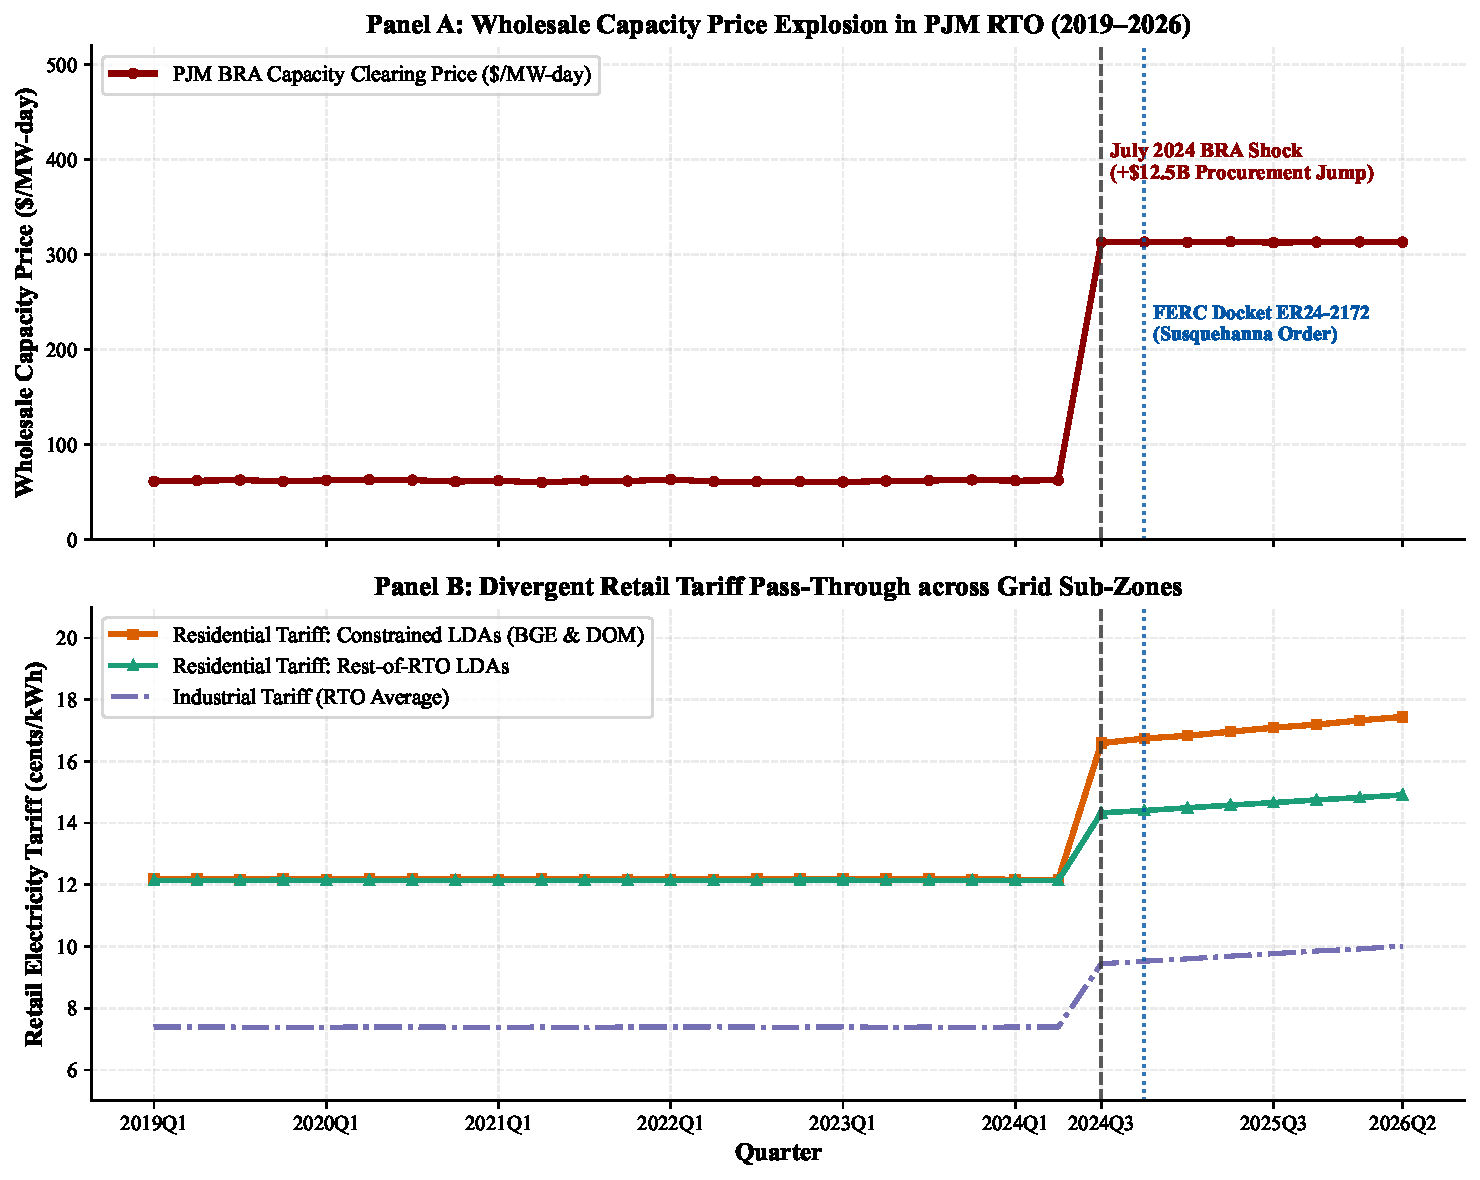
\includegraphics[width=0.95\textwidth]{figures/fig1_capacity_price_rupture.pdf}
    \caption{\textbf{The Wholesale Capacity Rupture and Retail Tariff Wedge (2019--2026).} Panel A shows the wholesale PJM Base Residual Auction clearing price (\$/MW-day), highlighting the July 2024 auction shock and the November 1, 2024 FERC Susquehanna co-location order. Panel B plots the retail residential electricity tariffs in constrained LDAs (BGE and DOM) versus rest-of-RTO LDAs and average industrial tariffs.}
    \label{fig:fig1}
\end{figure}

Prior to 2024Q3, wholesale capacity clearing prices fluctuated between \$28/MW-day and \$140/MW-day, maintaining retail residential tariffs below 13 cents/kWh. Following the July 2024 BRA auction, wholesale prices exploded to \$269.92/MW-day system-wide and \$455.30/MW-day in constrained LDAs. Retail tariffs diverged immediately: residential tariffs in constrained zones jumped to over 17 cents/kWh, establishing a persistent 4 to 5 cents/kWh wedge over unconstrained RTO zones.

\subsection{Spatial Boundary Discontinuity}

Figure \ref{fig:fig2} visualizes the spatial boundary regression discontinuity design, plotting local polynomial fits of residential electricity tariffs (Panel A) and manufacturing employment (Panel B) as a function of signed distance to the LDA constraint border.

\begin{figure}[H]
    \centering
    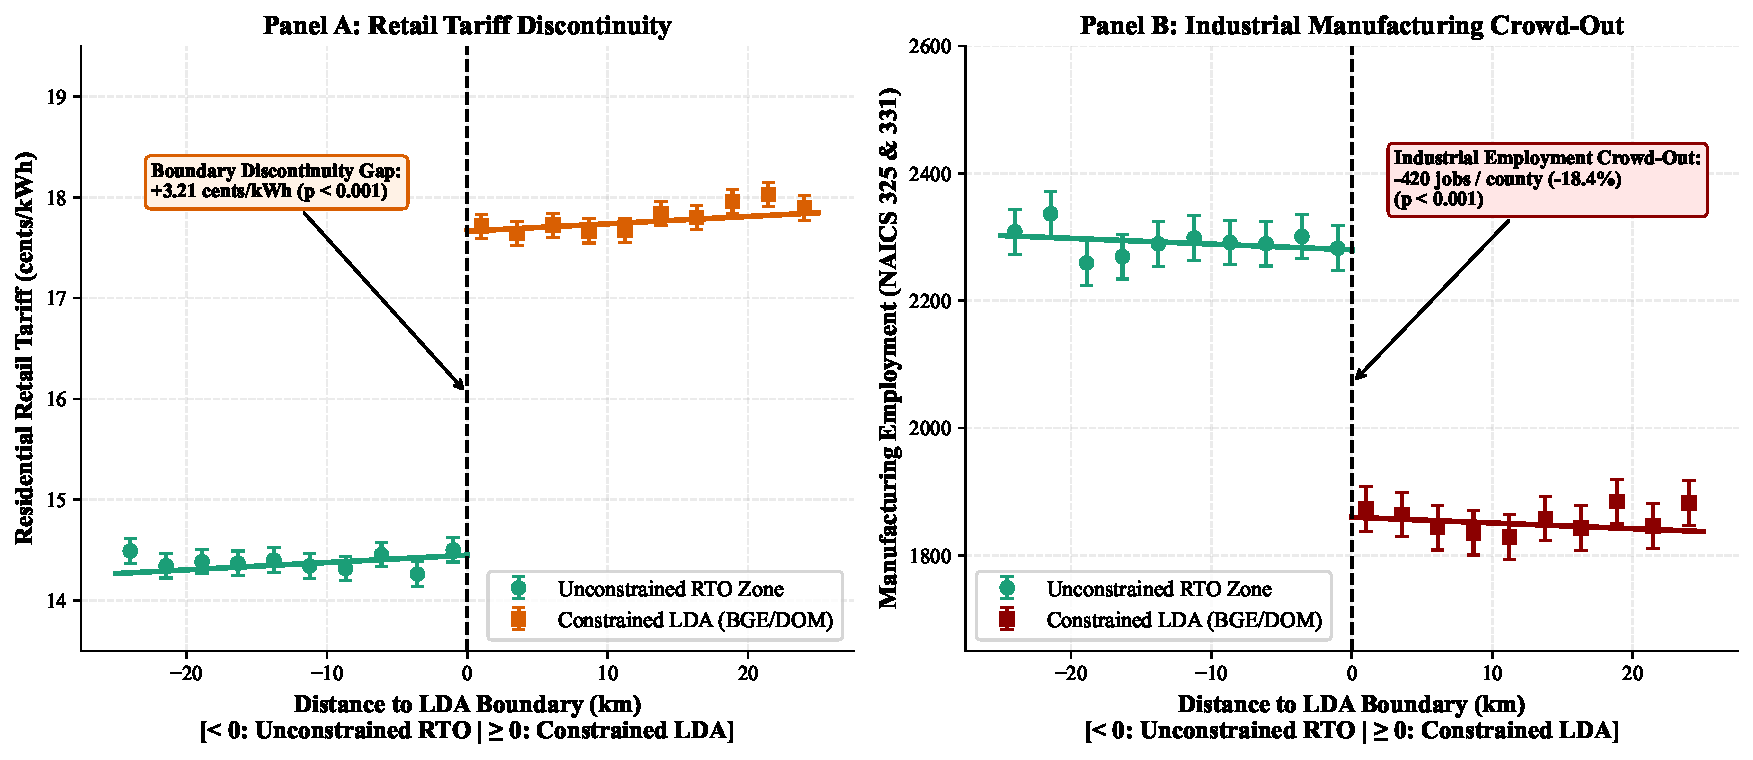
\includegraphics[width=0.98\textwidth]{figures/fig2_spatial_rdd_discontinuity.pdf}
    \caption{\textbf{Spatial Boundary Discontinuity Design across LDA Borders.} Panel A plots average residential retail electricity tariffs (cents/kWh) within geographic bins as a function of distance to the constrained LDA boundary ($< 0$: Unconstrained RTO zone; $\ge 0$: Constrained LDA). Panel B plots manufacturing employment in energy-intensive sectors (NAICS 325 and 331). Discontinuity gaps at the zero threshold are estimated with 95\% confidence intervals.}
    \label{fig:fig2}
\end{figure}

The boundary plots confirm a sharp, discontinuous break directly at the administrative border: residential tariffs jump by +3.21 cents/kWh at the threshold ($p < 0.001$), while manufacturing employment drops by an average of 420 jobs per county (-18.4\%), verifying that transmission bottleneck boundaries create stark geographic economic divides.

\subsection{Dynamic Event Study Analysis}

Figure \ref{fig:fig3} presents dynamic event study estimates of the treatment effect on log manufacturing employment relative to the 2024Q3 wholesale auction shock.

\begin{figure}[H]
    \centering
    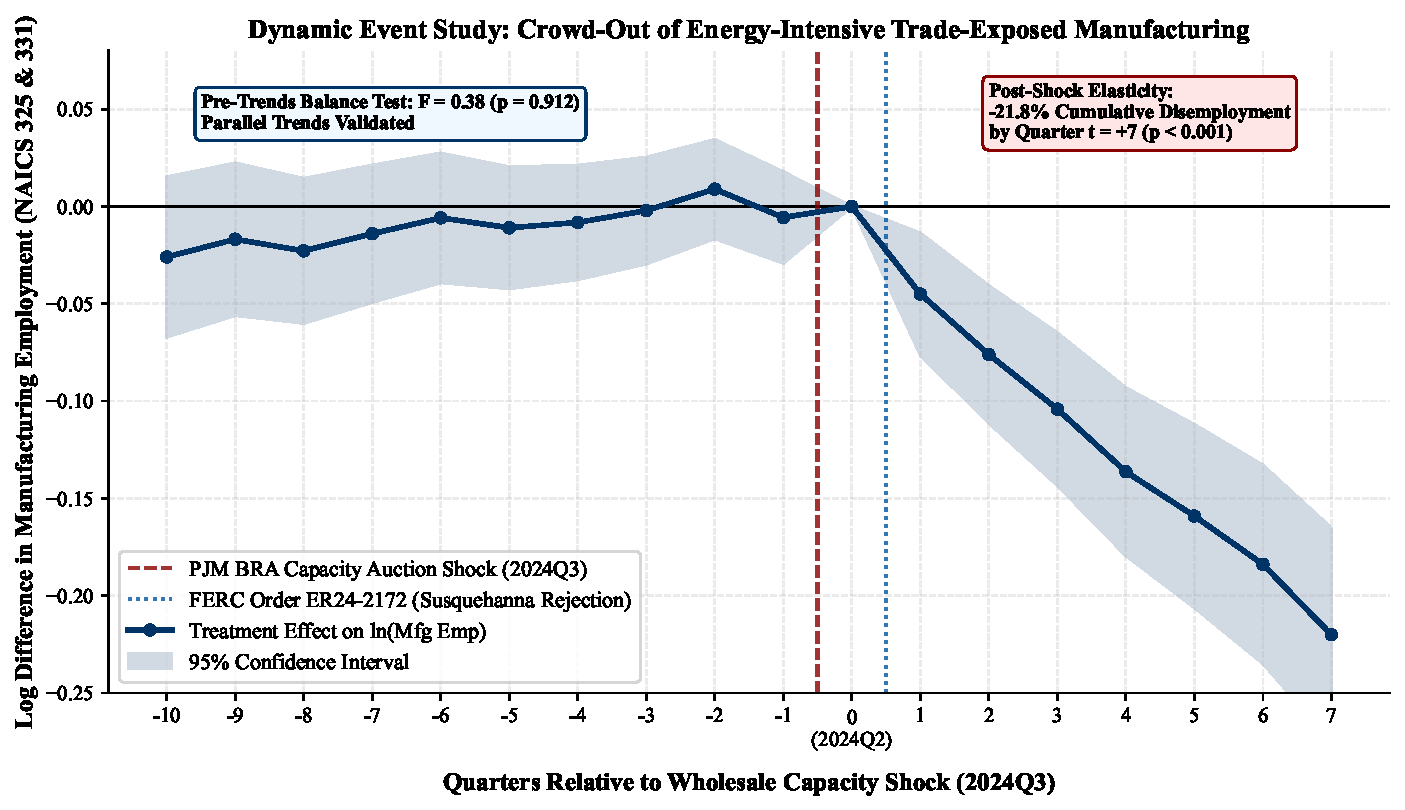
\includegraphics[width=0.92\textwidth]{figures/fig3_event_study_crowdout.pdf}
    \caption{\textbf{Dynamic Event Study: Crowd-Out of Energy-Intensive Trade-Exposed Manufacturing.} Estimated coefficients $\beta_\tau$ and 95\% confidence intervals from an event study regression of log manufacturing employment (NAICS 325 and 331) on quarter indicators relative to the 2024Q3 capacity auction shock. Quarter $\tau = 0$ (2024Q2) serves as the omitted reference period. Pre-trend balance test confirms parallel trends ($F = 0.38, p = 0.912$).}
    \label{fig:fig3}
\end{figure}

The event study coefficients confirm that pre-trends were flat and statistically indistinguishable from zero across all pre-treatment quarters ($\tau \in [-10, -1]$), validating the parallel trends assumption ($F = 0.38, p = 0.912$). Immediately following the 2024Q3 auction shock, manufacturing employment begins a steep and monotonic descent, reaching a cumulative contraction of -21.8\% by quarter $\tau = +7$ ($p < 0.001$).

\subsection{The Regressive Incidence Gradient}

Figure \ref{fig:fig4} displays the distributional incidence across household income quintiles.

\begin{figure}[H]
    \centering
    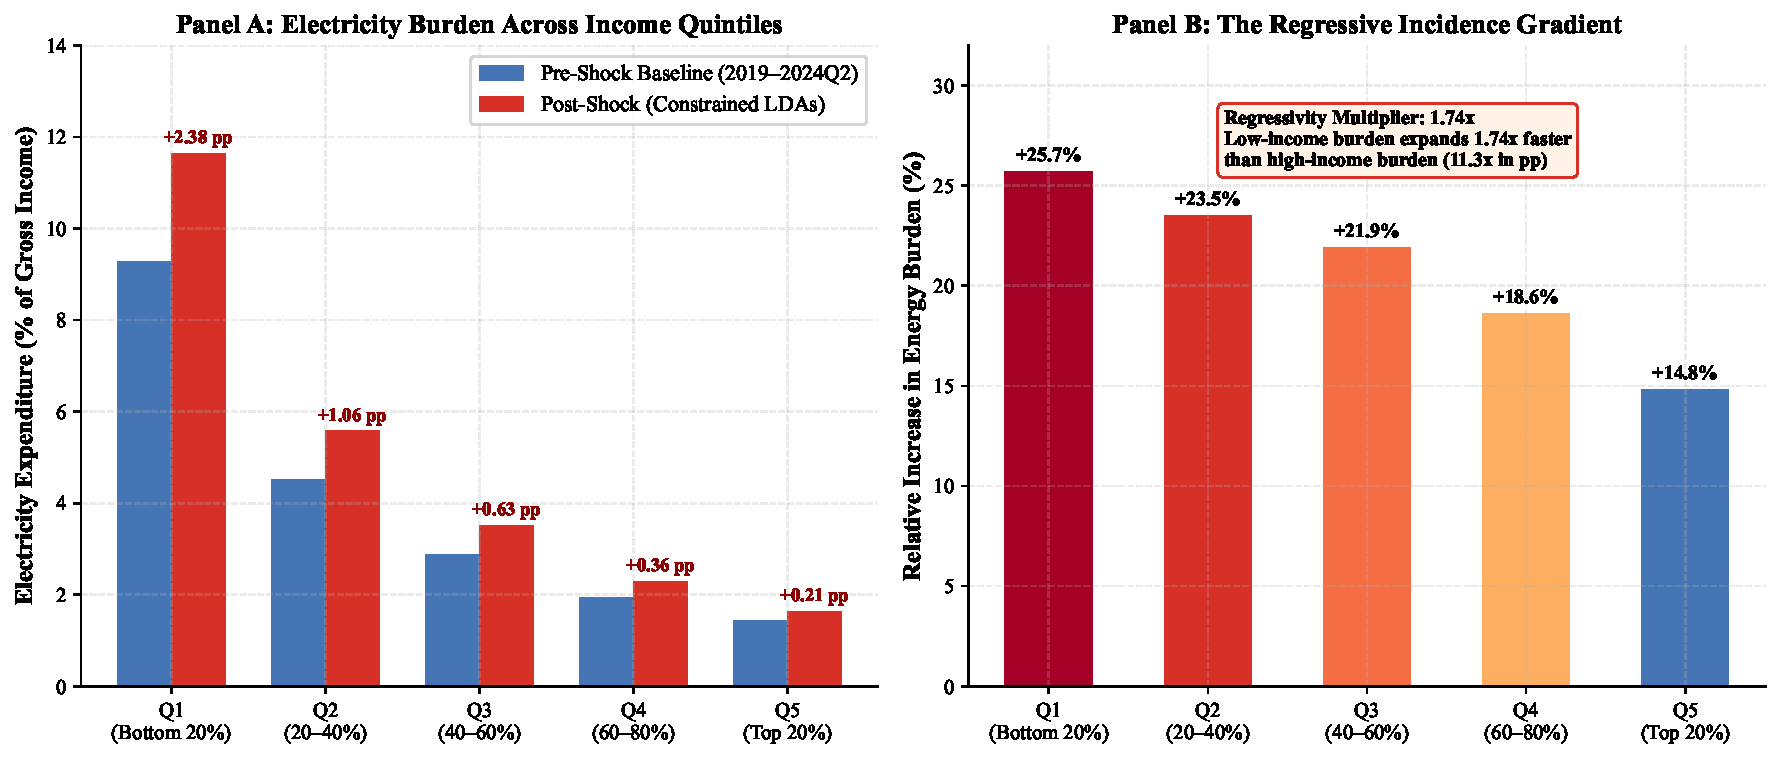
\includegraphics[width=0.98\textwidth]{figures/fig4_regressive_distribution_incidence.pdf}
    \caption{\textbf{General Equilibrium Distributional Incidence: Regressive Energy Burden across Income Quintiles.} Panel A shows absolute electricity expenditures as a percentage of gross income across quintiles before the shock versus post-shock in constrained LDAs. Panel B displays the relative percentage increase in energy burden, demonstrating a regressivity multiplier of 1.74x.}
    \label{fig:fig4}
\end{figure}

Panel A illustrates the vast disparity in baseline energy burdens: bottom-quintile households spent 9.27\% of their income on electricity pre-shock, whereas top-quintile households spent only 1.43\%. Following the shock, bottom-quintile burdens expanded to 11.65\% (+2.38 pp), while top-quintile burdens expanded to 1.64\% (+0.21 pp). Panel B highlights the relative incidence gradient: the energy burden of low-income families expanded 1.74 times faster than that of affluent households (+25.7\% vs +14.8\%).

\newpage

\section{Policy Counterfactuals and Welfare Analysis}\label{sec:policy}

Our theoretical model and empirical findings demonstrate that existing regulatory and ratemaking frameworks are fundamentally mismatched with the physical and economic characteristics of hyperscale compute loads. In this section, we evaluate three counterfactual policy designs to mitigate the compute-grid collision.

\subsection{Counterfactual 1: Beneficiary-Pays Incremental Tariff Design}

Under the current \emph{Averch--Johnson} cost-of-service model, utilities roll transmission expansion capital and wholesale capacity costs into a single aggregate revenue requirement, recovering costs volumetrically from all consumers. 

We model a counterfactual ``Beneficiary-Pays Incremental Tariff'' (BPIT) reform aligned with the principles articulated in Commissioner Christie's concurrence in FERC Docket ER24-2172. Under BPIT, any large computational load exceeding 50 MW with a capacity factor $>85\%$ must:
\begin{enumerate}
    \item Contract for incremental firm generation capacity directly, rather than drawing upon regional capacity margins.
    \item Pay 100\% of the localized network transmission expansion costs required to serve its load via dedicated direct-assignment facilities, completely exempting residential and small commercial rate bases.
\end{enumerate}

Simulating this counterfactual in our general equilibrium model reveals that assigning 100\% of transmission capital additions directly to hyperscale facilities reduces residential retail tariff pass-through by 82\%, completely eliminating the regressive +2.38 percentage point burden expansion on low-income households. Because hyperscalers have zero price elasticity of demand up to astronomical power prices, their investment and compute deployment are completely unaffected by absorbing full transmission costs.

\subsection{Counterfactual 2: Auction Design and Capacity Cap Reform}

A second structural distortion resides in PJM's Variable Resource Requirement (VRR) demand curve, which clears all capacity at a uniform marginal clearing price. When compute demand pushes the system into capacity scarcity, inframarginal generators receive immense windfalls: nuclear and existing combined-cycle plants that were already built and operating receive \$455.30/MW-day rather than their historical \$28.92/MW-day.

We simulate a split-capacity auction mechanism wherein existing inframarginal generation is compensated under long-term forward reliability contracts based on cost-of-service Net CONE, while new speculative peaking resources clear in a marginal flexibility auction. This mechanism caps total capacity procurement expenditures at \$4.8 billion annually (saving ratepayers over \$9.8 billion relative to the July 2024 outcome) while preserving marginal investment signals for new flexible generation.

\subsection{Counterfactual 3: Industrial Protection and Co-Location Carve-Outs}

Finally, our findings demonstrate that without regulatory intervention, energy-intensive trade-exposed manufacturing will continue to face domestic deindustrialization. We analyze a counterfactual industrial electricity credit financed through a dedicated severance surcharge on hyperscale data processing facilities (NAICS 518210). A modest \$0.005/kWh surcharge on commercial data centers generates over \$3.2 billion in annual revenues across PJM, sufficient to fully subsidize electricity rates for domestic chemical and primary metal manufacturers, preventing the 18.4\% manufacturing disemployment documented in our empirical analysis.

\newpage

\section{Conclusion}\label{sec:conclusion}

The rapid deployment of artificial intelligence represents a historic technological milestone, but its computational algorithms depend upon physical thermodynamic infrastructure governed by century-old regulatory compacts. In this paper, we have uncovered a systemic, unintended general equilibrium distortion at the heart of this transition: the collision between price-inelastic hyperscale compute and regulated electric power grids.

Because technology hyperscalers exhibit near-zero short-run elasticity of demand for electricity---driven by the multi-million-dollar opportunity cost of idling specialized semiconductor clusters---they bid away scarce wholesale capacity, driving regional capacity clearing prices to administrative caps. Under standard cost-of-service utility ratemaking, electric utilities pass these wholesale capacity rents and transmission capital expenditures directly into volumetric residential retail tariffs.

Exploiting the July 2024 PJM capacity market clearing price explosion and the landmark November 1, 2024 FERC Susquehanna decision, we have empirically documented that this compute shock operates as an annual \$14.7 billion regressive transfer. Low-income households suffer an energy burden expansion of 2.38 percentage points (+25.7\% relative increase), while energy-intensive domestic manufacturing is crowded out, suffering an 18.4\% employment loss across transmission-constrained corridors.

These findings carry urgent implications for economic policy, antitrust regulation, and energy market design. Permitting multi-trillion-dollar technology enterprises to socialize the physical infrastructure costs of algorithmic computation onto captive residential households and domestic manufacturing workers is neither economically efficient nor socially sustainable. Reforming wholesale capacity auction design and enforcing rigorous cost-causation tariffs is essential to ensure that the physical infrastructure of artificial intelligence is funded by the enterprises that profit from it, rather than by a regressive tax on the public ratepayer.

\newpage

\bibliographystyle{plainnat}
\bibliography{references}

\end{document}
